\section{Theorie}
\label{sec:Theorie}

\subsection{Interferenz, Kohärenz und Polarisation}
\label{sec:polarisation}
Licht wird in diesem Versuch als elektromagnetische Welle betrachtet, um Interferenzerscheinungen erklären zu können. Die elektrische Feldstärke ist 
ebenfalls eine solche Welle und kann über 
\begin{equation}
    \vec{E} = \vec{E}_0\cos{(\vec{k}\cdot \vec{r}+\omega t+ \delta)}
    \label{eqn:EVektor}
\end{equation}
beschrieben werden. Der Vektor $\vec{E}$ beschreibt die Amplitude in die drei Raumrichtungen und $\vec{k}$ ist der Wellenvektor, $\vec{r}$ ist die Ausbreitungsrichtung, $\omega$ steht für die Kreisfrequenz des Lichtes, $t$ stellt die Zeit dar und die Phase wird durch $\delta$ beschrieben. Informationen über Polarisation, auf die später noch eingegangen wird, werden von $\vec{E}$ getragen. Für Licht mit der Ausbreitungsrichtung in $z$-Richtung und linearer Polarisation in $x$-Richtung folgt
\begin{align*}
    \vec{r}&= \left(\begin{array}{c}0 \\ 0 \\ z\end{array}\right) \; ,\\
    \vec{E}&= \left(\begin{array}{c} E_0 \\ 0 \\ 0\end{array}\right)\; .
\end{align*}

Die Ausbreitung von Licht wird dabei über die Maxwellschen Gleichungen beschrieben. Außerdem folgt das elektrische Feld 
$\vec{E}$ dem Prinzip der linearen Superposition.
Die Intensität berechnet sich durch 
\begin{equation*}
    I = \langle E^2\rangle _{\text{T}} \; ,
\end{equation*}
wobei $\langle E^2\rangle _{\text{T}}$ nichts anderes als der zeitliche Mittelwert in einem Intervall T ist
\begin{equation}
    \langle f(t) \rangle _{\text{T}} = \frac{1}{T}\int_t^{t+T} f(t')\text{d}t \, .
    \label{eqn:zeitlichMittel}
\end{equation}
Da $E$ aus einer Überlagerung von zwei Wellen besteht, wird $\vec{E}=(\vec{E}_1+\vec{E}_2)$ gesetzt, wodurch $\vec{E}^2= E_1^2+E_2^2+2\vec{E_1}\, \vec{E}_2\cdot\text{cos}(\alpha)$ folgt.
Der Winkel $\alpha$ ist hierbei der Winkelzwischen den beiden Wellen.
Bei einer Überlagerung von zwei Wellen ergibt sich für die Intensität 
\begin{equation*}
    I = I_1 +I_2 +I_{12}\; .
\end{equation*}
Der Ausdruck $I_{12}$ beschreibt hierbei den Interferenzterm.
Nimmt man an, dass $I_1=I_2$ gilt, so folgt, dass
wenn die Bedingung
\begin{equation*}
    \delta_2 -\delta_1 = \left(2n+1\right)\pi 
\end{equation*}
erfüllt ist, sich die Intensität zu null ergibt und
bei 
\begin{equation*}
    \delta_2 -\delta_1 = \left(2n\right)\pi 
\end{equation*}
sich ein Intesitätsmaximum der Stärke $I=4I_1cos^2{\left(\frac{\delta}{2}\right)}$ zeigt.

Bei zwei unabhängigen Lichtquellen, sind die Phasenkonstanten $\delta_1$ und $\delta_2$ statistische Funktionen der Zeit, wodurch es keine 
Interferenzerscheinung gibt. Dieses Licht ist dann inkohärent. Mithilfe eines LASERs (light amplification by stimulated emission of radiation)
ist es jedoch möglich kohärentes Licht zu erzeugen, welches ein festes $k$, $\omega$ und $\delta$ besitzt.
Bei einem Wegunterschied der einzelnen Strecken des Interferometers, der der Kohärenzlänge $l$ oder mehr entspricht, verschwindet jedoch die 
Interferenzerscheinung. Die Kohärenzlänge berechnet sich über
\begin{equation*}
    l = \text{N}\lambda \; .
\end{equation*}
Dabei ist N die Anzahl der bei beobachtbaren Intensitätsmaxima. Die Anzahl der beobachteten Maxima entsteht durch den Wegunterschied. Wenn der Welle ein Wegunterschied von $\Delta s=\lambda$ widerfährt, so ist ein Maximum erkennbar.Bei zweifachem Wegunterschied sind zwei Maxima detektierbar usw.
Diese Eigenschaft wird für die Bestimmung des Brechungsindex von Glas und Luft verwendet (siehe \autoref{sec:Durchführung}).

Eine weitere wichtige Eigenschaft für die Interferenz von Licht ist die Polarisation. Lichtpolarisation kann in vier Hauptkategorien unterteilt werden. Die erste ist die lineare Polarisation, bei der die Schwingungsrichtung des elektrischen Feldvektors in einer einzigen Ebene liegt.
 Darüber hinaus gibt es die zirkulare Polarisation. Hierbei rotiert die Schwingungsrichtung des elektrischen Feldvektors in einer kreisförmigen Bewegung. Die Schwingrichtung liegt folglich nicht mehr nur in einer Ebene. Zirkular Polarisiertes Licht kann weiter in zwei Unterkategorien unterteilt werden; links und
 rechtshändig polarisiert. Diese Polarisationsrichtung beschreibt die Richtung der Schwingung in Abhängigkeit zur Ausbreitungsrichtung 
Die dritte Möglichkeit ist die elliptische Polarisation, die eine Kombination aus linearer und zirkularer Polarisation ist. Bei dieser Art der Polarisation rotiert die Schwingungsrichtung des Feldvektors in einer elliptischen Bewegung.
Die letzte Möglichkeit ist unpolarisiertes Licht, welches sich durch keine geordnete Schwingungsrichtung auszeichnet.  
Drei der genannten Möglichkeiten sind in \autoref{fig:polarisation1} schematisch dargestellt.

\begin{figure}
    \centering
   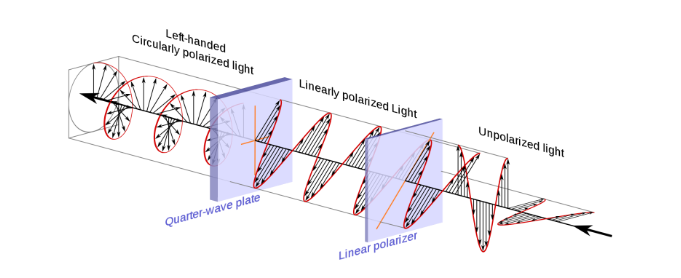
\includegraphics[width = 0.7 \linewidth]{Bilder/polarisation1.png}
    \caption{Drei der möglichen Polarisationsarten und Möglichkeiten diese ineinander umzuwandeln. \cite{Polarisation}.}
    \label{fig:polarisation1}
\end{figure}
Um ein Interferenzmuster zu erhalten, ist es nötig dass die Polarisationsrichtung der beiden Teilstrahlen nicht senkrecht aufeinander stehen. Für ein möglichst deutliches Interferenzmuster müssen beide Wellen die gleiche Polarisationsrichtung und -art haben.

\subsection{Kontrast} \label{sec:kontrast}
Als Kontrast (oder Sichtbarkeit) eines Interferometers wird die Beziehung
\begin{equation} \label{eqn:kontrast}
    V = \frac{I_\text{max} - I_\text{min}}{I_\text{max} + I_\text{min}}
\end{equation}
bezeichnet. Offensichtlich gilt also für den Kontrast: $V \in [0,1]$.
Hierbei beschreibt $V$ die Qualität und Deutlichkeit des Interferenzbildes. Hat $V$ den Wert 1, so ist das Minimum nicht sichtbar. Je stärker das Minimum sichtbar ist, desto kleiner wird $V$ bis es den Wert 0 erreicht und keine Interferenz mehr zu erkennen ist.
Aus zwei überlagerten Wellen $E=(E_1+E_2)$ folgt nach Einsetzen von \autoref{eqn:EVektor} in \autoref{eqn:zeitlichMittel} für die Intensität
\begin{equation*}
    I = \langle E^2\rangle _{\text{T}}= \frac{1}{T}\int_t^{t+T}  (\vec{E}_{0,1}\cos{(\omega t)})^2+(\vec{E}_{0,2}\cos{(\omega t+ \delta)})^2+2\vec{E}_{0,1}\cos{(\omega t)}\, \vec{E}_{0,2}\cos{(\omega t+ \delta)}\cdot\text{cos}(\alpha)\text{d}t\, .
\end{equation*}
Hierbei wurde die Phasenverschiebung $\delta$ als Verschiebung der zweiten zur ersten Welle definiert. Unter der Vereinfachung, dass sich die Welle nur entlang einer Achse ausbreitet, der Winkel zwischen den beiden Strahlen $\alpha=0$ ist und beide Wellen die gleiche Intensität haben folgt für die Intensität

\begin{equation*}
    I=\frac{1}{T}\int_t^{t+T} (E_{0}\cos{(\omega t)})^2+(E_{0,2}\cos{(\omega t+ \delta)})^2+2E_{0}\cos{(\omega t)}\, E_{0}\cos{(\omega t+ \delta)}\text{d}t\, .
\end{equation*}
Nach nach kurzer Umformung kann 
folgende Proportionalität für die Intensitätsmaxima/- und minima gefunden werden
\begin{equation*}
    I_\text{max/min} \propto I_\text{Laser} \left[ 1 \pm 2 \cos(\Phi) \sin (\Phi) \right] \, ,
\end{equation*}
aus der sich wiederrum mit \autoref{eqn:kontrast} die Gleichung
\begin{align}\label{eqn:kontrast2}
    V = V(\Phi) &\propto \left|\frac{\left[ 1 + 2 \cos(\Phi) \sin (\Phi) \right] - \left[ 1 - 2 \cos(\Phi) \sin (\Phi) \right]}{\left[ 1 + 2 \cos(\Phi) \sin (\Phi) \right] + \left[ 1 - 2 \cos(\Phi) \sin (\Phi) \right]}\right| \\
    &= \left|2 \cos(\Phi) \sin(\Phi) \right| = \left| \sin (2 \Phi) \right|
\end{align}
ergibt. %Hieraus ist auch sofort ersichtlich, dass der Kontrast bei ungefähr $45°$ am höchsten sein dürfte, wenn alle anderen Einflüsse optimiert sind.
Die Größe $\Phi$ ist hierbei der Polarisationswinkel. 
\subsection{Brechungsindex} \label{sec:n}

Der Brechungsindex ist eine intrinsische Eigenschaft eines Materials und kann mittels Interferometer bestimmt werden. Ein Medium mit einem Brechungsindex $n_\text{Medium} > 1$ reduziert die Geschwindigkeit des einfallenden Lichts, was durch die Gleichung
\begin{equation*}
    v_\text{Medium} = \frac{c}{n}
\end{equation*}
beschrieben wird. Ein Lichtstrahl, der durch ein Medium geleitet wird, erfährt eine Phasenverschiebung. Diese Phasenverschiebung kann in Interferometern genutzt werden, um den Brechungsindex eines Mediums zu bestimmen.

Für die Phasenverschiebung in Luft gilt
\begin{equation} \label{eq:nluft}
    \Delta \delta = \frac{2 \pi}{\lambda_\text{vac}} \Delta n \cdot L \, ,
\end{equation}
wobei $L$ die Länge der evakuierten Zelle ist. Durch Einsetzen der Beziehung der gezählten Intensitätsmaxima 
\begin{equation} \label{eq:maxima}
    M = \frac{\Delta \delta}{2 \pi}
\end{equation}
in \autoref{eq:nluft} lässt sich der Brechungsindex bestimmen:
\begin{align} \label{eq:nluft2}
    \Delta n &= n_\text{Luft} - n_\text{Vak} = \frac{M \cdot \lambda_\text{vac}}{L} \nonumber \\
    n_\text{Luft} &= \frac{M \cdot \lambda_\text{vac}}{L} + 1
\end{align}

Mithilfe des Lorentz-Lorenz-Gesetzes lässt sich der Brechungsindex unter Normalbedingungen berechnen. Das Lorentz-Lorenz-Gesetz lautet
\begin{equation*}
    \frac{n^2 - 1}{n^2 + 2} = \frac{A p}{R T} \, ,
\end{equation*}
wobei $A$ die Refraktivität beschreibt und $R$ die allgemeine Gaskonstante. Nach einer Taylorentwicklung ergibt sich
\begin{equation*}
    n(p) \approx \frac{2 (n-1)}{3} \, ,
\end{equation*} 
woraus sich dann
\begin{equation} \label{eq:lorentz}
    n (T,p) \approx \frac{3 A p}{ 2 R T} + 1
\end{equation}
ergibt. Die Größe $T$ ist hierbei die Temperatur.

In diesem Experiment wird auch der Brechungsindex von Glas bestimmt. Für den Brechungsindex in Glas gilt
\begin{equation}\label{eq:phiglas}
    \Delta \phi = \frac{2\pi}{\lambda}T\left(\frac{n-1}{2n}\Delta \theta^2+O( \Delta \theta^4)\right) \, .
\end{equation}
Hierbei ist $T$ die Dicke des Glasplättchens.
Diese Gleichung wird modifiziert, da zwei Glasplättchen verbaut sind und um $\theta_0 = \pm 0.175\,\text{rad}$ verkippt sind. Damit ergibt sich die Gleichung in führender Ordnung
\begin{equation}
    \Delta \phi = \frac{\pi \cdot (n - 1) T}{\lambda \cdot n} \left(\left( \theta + 0.175 \right)^2 - \left( \theta - 0.175 \right)^2\right) \, ,
\end{equation}
was mit \autoref{eq:maxima} auf die Gleichung
\begin{equation*}
    M = \frac{n - 1}{\lambda \cdot n} \cdot 2 \theta \cdot |\theta_0|
\end{equation*}
und somit auf
\begin{equation} \label{eq:n_Glas}
    n = \frac{1}{1- \frac{\lambda M}{ 2 \theta \cdot |\theta_0| T}}
\end{equation}
führt.